\chapter{Design \& Implementering}

Dette afsnit beskriver overvejelser omkring valg af design, diagrammer vedrøende implementering

\section{Design}
Da vi skulle lave vores design stod vi mellem to mulidheder. Enten skulle det være ren activity baseret eller baseret på en tab menu med få activities. \\
Vi tænkte at det ville være en dårlig bruger oplevelse at man konstant hoppede rundt i activities, og valgte derfor at få med den tab basrede udgave.
Her under ses et billede af hvordan vores Homescreen ser ud i Shine My Room

\begin{figure}[H]
	\centering
	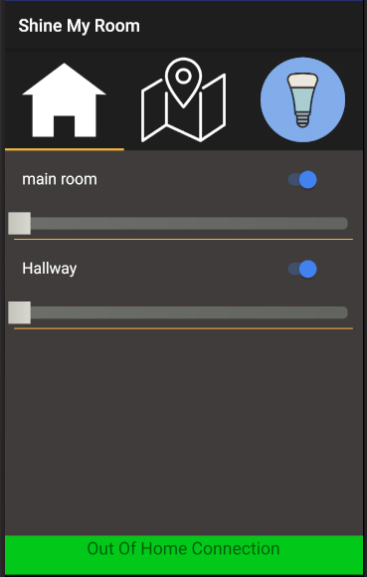
\includegraphics[width=0.5\linewidth, height=0.7\linewidth]{Design/Startscreen}
	\caption{Startscreen}
	\label{fig:Startscreen}
\end{figure}
Applikationen er bygget op af en tab baseret activity hvor der ligger tre tabs man som standard kan hoppe rundt i mellem. Under disse ligger der forskellige fragments som f.eks. listen af rooms som kan ses på billedet. Her kan man se navnet på et af de rum man har oprettede, tænde for pærene som er connected til rummet og bestemme lysstyrken på pærene.


\section{UML diagram}
Her under ses UML diagrammet for Shine My Room
\begin{figure}[H]
	\centering
	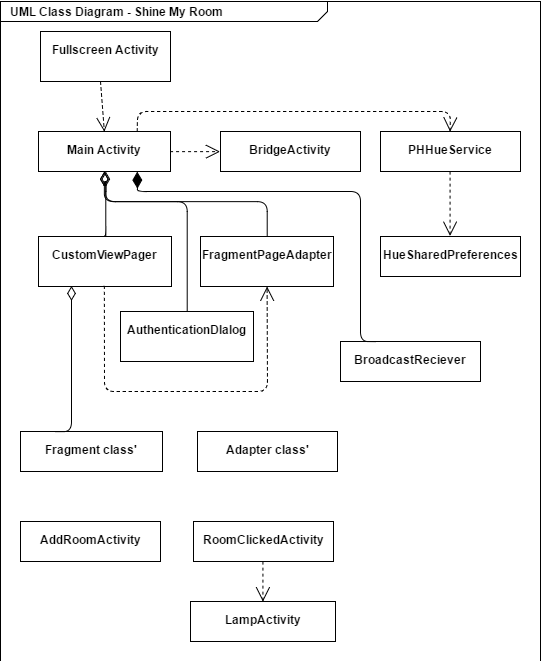
\includegraphics[width=0.6\linewidth, height=0.7\linewidth]{Design/UMLDiagram}
	\caption{UML}
	\label{fig:UML Diagram}
\end{figure}
For at holde UML diagrammet simpelt uden for mange dependencies har vi samlet vores fragment class' og adapter class' i en. \\
Vores fragment class' består altså af klasserne: EditRoomFragment, GeoFencingFragment, LoadingFragment, NoBridgeConnectFragment og RoomListFragment.\\
Adapter class' består af: AddRoomAdapter, EditRoomAdapter, FragmentPageAdapter, RemoteRoomAdapter, RoomAdapter og RoomClickedAdapter.

De activities som ligger i bunden er lagt ind på denne måde, da de udspringer af en fragment, og derfor kunne vi ikke placere deres dependensy pga den samlede fragment class.
\newpage

\section{Sekvensdiagram}
Her under ses sekvensdiagrammet for Shine My Room
\begin{figure}[H]
	\centering
	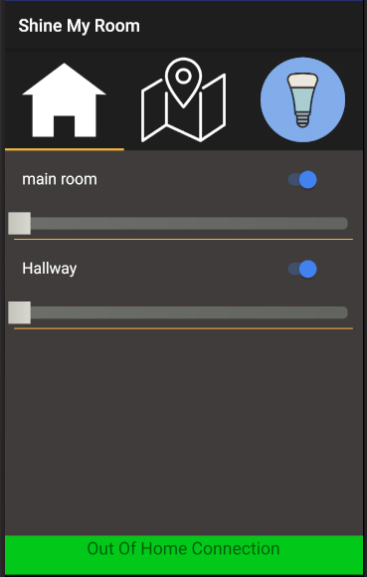
\includegraphics[width=0.5\linewidth, height=0.7\linewidth]{Design/Startscreen}
	\caption{Sekvensdiagram}
	\label{fig:Sekvensdiagram}
\end{figure}